\section{Einleitung}
\label{s:intro}

\section{Vorgestellte Technologien}
\label{s:grundlagen}

Im folgenden Kapitel wird einleitend eine kurze Erläuterung über die drei zentralen Begriffe dieser Arbeit gegeben. Besonderer Schwerpunkt ist dabei die Aufschlüsselung der Begriffe und die Erklärung warum Diese in dieser Arbeit einen derartigen Stellenwert besitzen.\\ 

\subsection{IoT}
\label{ss:grundlagen:beispiele}


\subsection{Industrie 4.0}
\label{ss:grundlagen:hardware}


\subsection{SAP}
\label{ss:grundlagen:frequenz}


\section{Allgemeine Funktionsweise Bluetooth Low Energy}
\label{s:funktionsweise}

\noindent Im nachfolgenden Kapitel wird nun ein kurzer Überblick über die Technologie \ac{ble} gegeben. Dabei wird zum einen die Architektur unter Erläuterung des Protokollstacks und zum anderen die Funktionsweise erläutert.\\   

\subsection{Protokollstack}
\label{ss:funktionsweise:protokollstack}

\begin{figure}[!b]
	\centering
	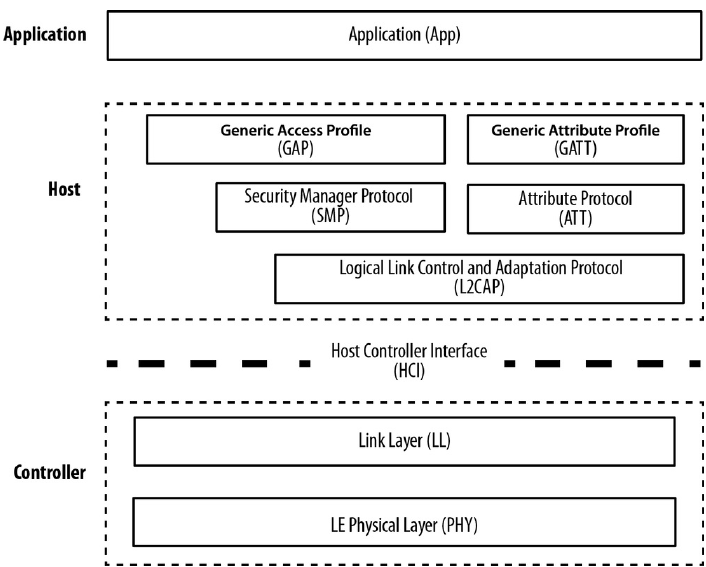
\includegraphics[width=0.6\linewidth]{\figdir/BLE_Protokolstack}
	\caption{\ac{ble} Protokollstack \cite[Seite 16]{Townsend14:GSB}}
	\label{FIG:protokollstack}
\end{figure}

\noindent Die Architektur von \ac{ble} geht aus dem Protokollstack hervor. Dieser ist in Abbildung \ref{FIG:protokollstack} dargestellt. Besonders auffällig ist die Untergliederung in drei Ebenen. Der "`Controller"' stellt dabei den hardwarenähesten Bereich dar. Hier befinden sich die zwei Layer "`LE Physical"' und "`Link"'.\\

\noindent Diese beiden Protokolle sind in einer Großzahl von Gerätearchitekturen beheimatet. Das Physical Layer ist dafür vorgesehen, digitale Signale (Bitfolgen) in analoge umzuwandeln. Dieser Schritt wird benötigt, um die \ac{ble} Signale für etwaige Empfänger zugänglich zu machen. Natürlich werden im Physical Layer auch empfangene analoge Signale in digitale umgewandelt. Dieser werden dann im Protokollstack nach oben ins Link Layer weitergereicht. Im Fall von \ac{ble} ist die Schnittstelle für das Senden der analogen Signale die Luft. \ac{ble} sendet daher im Frequenzbereich 2,4GHz bis 2,4835GHz. Diesen Bereich teilt sich das Protokoll mit anderen wie beispielsweise Wifi. Um Kollisionen zu vermeiden teilt \ac{ble} den Bereich in 40 Kanäle auf und wechselt während der Verbindung in regelmäßigen Abständen oder bei Übertragungsproblemen den Kanal. Dieser Ansatz nennt sich Frequency Hopping Spread Spectrum \cite[Seite 16f]{Townsend14:GSB}.\\      

\noindent Das Link Layer unterscheidet sich in seiner Funktionsweise nicht großartig von dem anderer Kommunikationsprotokolle. Hier werden die Nachrichten die für das  Versenden aus den oberen Schichten ankommen in Pakete gepackt und an das Physical Layer weitergereicht. Dieser Prozess ist für ankommende Pakete natürlich vice versa \cite[Seit 194]{Tanenbaum14:CN}. Besonders wichtig ist die Festlegung der Paketgröße von \ac{ble} durch das Link Layer. Seit Version 4.2 ist eine Payload von bis zu 251 Byte pro Paket möglich \cite{Gupta:WWW}. Zum Vergleich bei WLAN (IEEE 802.11) kann ein Paket bis zu 2312 Byte groß sein \cite[Seite 233]{Gessler15:WNN}. Daraus lässt sich schließen, dass \ac{ble} einen weitaus geringeren Datendurchsatz als WLAN hat. Allerdings liefert \ac{ble} wiederum andere Vorteile. Auf diese wird in Kapitel \ref{s:vergleich} näher eingegangen.\\

\noindent Das Herzstück des \ac{ble} Protokollstacks bilden die beiden Profile \ac{gap} und \ac{gatt}. Diese befinden sich wie in Abbildung \ref{FIG:protokollstack} zu erkennen im Host Bereich der Architektur. Die beiden Protokolle bilden die Schnittstelle zur tatsächlichen Anwendung mit welcher der Nutzer interagiert.\\

\noindent Das \ac{gap} ist dafür vorgesehen sämtliche Parameter der Verbindung zwischen den Geräten zu verwalten. Vom Verbindungsaufbau bis hin zur Kommunikation werden sämtliche Funktionen von diesem Profil bereitgestellt und abgehandelt.\\

\noindent Im Zuge der jeweiligen Konfiguration kann ein Gerät in \ac{ble} eine der folgenden vier Rollen annehmen:
\begin{itemize}
	\item{Broadcaster (Keine Verbindung)}
	\item{Observer (Keine Verbindung)}
	\item{Central (Verbindung)}
	\item{Peripheral (Verbindung)}
\end{itemize}   

\noindent In \ac{ble} ist es nicht festgeschrieben, dass Geräte ein Verbindung eingehen müssen um Informationen zu erhalten. Die Rollen des Broadcasters und Observers sind sogar ausschließlich ohne feste Verbindung zwischen den Geräten vorgesehen. Diese Funktion wird im allgemeinen gerne von \ac{ble} Beacons verwendet.\\

\noindent Ein Gerät welches als Broadcaster definiert ist sendet dauerhaft einen bestimmten Datensatz. Dabei ist zu keinem Zeitpunkt klar, ob Geräte in Reichweite sind, welche den Datensatz empfangen. Ein Gerät welches diese Daten lesen kann muss als Observer konfiguriert sein. Ein solcher scannt die drei Advertisement Kanäle von \ac{ble} dauerhaft nach Broadcastnachrichten. Falls er eine erhält ließt er diese und verwendet sie. Wichtig ist hierbei, dass der Observer keine Antwort auf eine Nachricht sendet.\\  

\noindent Sollte ein Gerät allerdings eine Verbindung eingehen, dann muss dieses als Central konfiguriert sein. Dies ist die gängigste Form des \ac{ble} Gerätes. So ist beispielsweise jedes Smartphone in der Regel als Central konfiguriert und kann Verbindungen zu Peripherals wie zum Beispiel \ac{ble} Kopfhörern aufnehmen. Dabei ist ein Central in der Regel sogar in der Lage mehrere Verbindungen zu selben Zeit einzugehen.\\

\noindent Ein Peripheral wiederum ist das Gegenstück zum Central, welches seine Verbindungsbereitschaft an sämtliche Geräte in Reichweite signalisiert. Im Fall einer aktiven Verbindung übernimmt das Central die Steuerung des Gerätes unter Berücksichtigung des Funktionsumfangs des Peripherals \cite[Seite 34]{Usama17:BBS}.\\

\noindent Das \ac{gap} ermöglicht es einem \ac{ble} Gerät zusätzlich seine Sichtbarkeit und Verbindungsbereitschaft gegenüber anderen Geräten über die Advertisement Kanäle mitzuteilen. Dafür wird auf dem Gerät ein Modus eingestellt welcher anschließend an alle Geräte in Reichweite mitgeteilt wird. Ein Modus ist dabei eng mir der Geräterolle verbunden. Ein Gerät kann folgende Modi annehmen \cite[Seite 35]{Townsend14:GSB}:
\begin{itemize}
	\item{Broadcast (Rolle: Broadcaster)}
	\item{Nicht zu entdecken (Rolle: Peripheral)}
	\item{Eingeschränkt zu entdecken (Rolle: Peripheral)}
	\item{Normal zu entdecken (Rolle: Peripheral)}
	\item{Nicht verbindbar (Rolle: Alle)}
	\item{Verbindbar (Rolle: Central, Peripheral)}
\end{itemize}   

\noindent Im \ac{gatt} wird definiert, ob es sich bei dem Gerät um einen Client oder Server handelt. Zweiterer verarbeitet die Kommunikationsanfragen des Clients und liefert die gewünschten Antworten oder führt entsprechende Aktionen aus. Der Server ist in der Regel ein Peripheral auf dem Services hinterlegt sind \cite[Seite 30]{Usama17:BBS}. Welche das sind und was für eine Aktion mit diesen verbunden ist wird in der Regel durch die Nutzeranwendung festgelegt. Der Client ist dementsprechend ein Central, welches die gesamte Verbindung steuert. Jeder Service verfügt über einen \ac{uuid}. Mit diesem kann der Client eine gezielte Anfrage auf den entsprechenden Service tätigen.\\    

\noindent An oberster Stelle des Protokollstacks befindet sich die Nutzeranwendung. Diese ist nach dem entsprechenden Use Case programmiert und variiert von Anwendung zu Anwendung. Ausschließlich der Stack unterhalb ist für alle Applikationen gleich.\\

\subsection{Kommunikation}
\label{ss:funktionsweise:kommunkation}

\noindent Nachdem in Kapitel \ref{ss:funktionsweise:protokollstack} der Aufbau von \ac{ble} erläutert wurde, wird nun in dem folgenden Kapitel auf die Anwendung der Technologie eingegangen. Dabei wird besonders auf den Verbindungsaufbau durch das Advertisement und den Nachrichtenaustausch der stehenden Verbindung eingegangen.\\

\subsubsection{Advertisement}
\label{sss:funktionsweise:advertisement}

Die Advertisement Funktion in \ac{ble} kann für zwei Szenarien verwendet werden. Zum einen die Signalisierung der Verbindungsbereitschaft. Zum anderen den Broadcast von Daten in der Rolle des Broadcasters (vgl. \ref{ss:funktionsweise:protokollstack}).\\

\noindent Von den 40 Kanälen, in die der \ac{ble} Frequenzbereich unterteilt ist, sind 3 für das Advertisement reserviert. Diese befinden sich in den Bereichen 2,402 - 2,404GHz, 2,426 - 2,428Ghz und 2,48 - 2,482GHz. Dabei sind sie mit den Nummern 37 - 39 belegt \cite[Seite 16]{Townsend14:GSB}.\\

\subsubsection{Verbindung}
\label{sss:funktionsweise:verbindung}   

\subsection{Anwendungsszenarien}
\label{ss:funktionsweise:anwendungen}

\section{Schnittstellenbeschreibung}
\label{s:interface} 

\subsection{SAP}
\label{ss:interface:sap}

\subsection{BLE}
\label{ss:interface:ble}

\subsection{Anbindungsmöglichkeiten}
\label{ss:interface:connect}

\subsubsection{Bewertung der Möglichkeiten}
\label{sss:interface:connect:eval}

\subsubsection{Administration}
\label{sss:interface:connect:admin}

\section{Vergleich mit anderen gängigen IoT Kommunikationsprotokollen}
\label{s:vergleich} 

\subsection{Vorteile}
\label{ss:vergleich:adv}

\subsection{Nachteile}
\label{ss:vergleich:disadv}

\section{Fazit}
\label{s:fazit}

  
%%% Local Variables: 
%%% mode: latex
%%% TeX-master: "thesis.tex"
%%% End: 
